David Rohrbaugh

2014-11-07

The Intake Mechanism, Samantha Module, and Electronics

\begin{tabular}{|p{5cm}|p{5cm}|}
 \hline
 This week, I worked on setting up the router and the flash drives for use with the driver station computer. The router used last year had to be reset and reconfigured. The flash drives also had to be made again. I have not been able to test my work because we are reconfiguring our robot's electronics to incorporate power poles.
 &
 All seems to be working properly as far as the Samantha Module is concerned. The robot's electronic parts with power poles incorporated are coming together.
 \\
 \hline
\end{tabular}

\medskip

This is a diagram of our current prototype for the intake mechanism. A Tetrix channel is attached to a DC motor so it rotates as shown. It is now geared up. The solid black portion is part of the robot's frame. The robot is facing to the right, with most of it to the left of this representation.

\begin{center}
 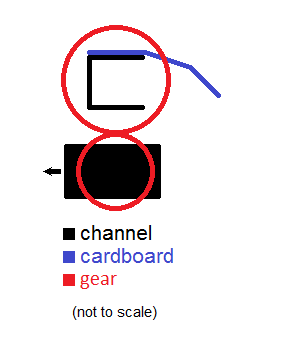
\includegraphics{./Entries/Images/intakePrototype2.png}
\end{center}
